\chapter{Method}
\label{ch:method}

\section{Datasets}
\label{ch:method-dataset}
This project focused on building an automated segmentation solution for radiotherapy. Two applications were targeted: A multi-organ segmentation model for pelvic imaging (with patient, bladder and rectum contouring); and a single structure model for vacuum bag contouring in canine imaging.\todo{maybe here add `as described in section blah'} Anonymised pelvic imaging data was provided by Riverina Cancer Care Centre from active prostate cancer RT patients over multiple stages of treatment. Canine imaging data was provided by the Small Animal Specialists Hospital (SASH) and contained variable cancer locations and patient orientations. All input data consisted of raw diagnostic CT images acquired with a 512 x 512 matrix. Pelvic imaging scans were comprised of 1.37 mm x 1.37 mm x 2 mm voxels; while canine imaging scans contained variable spacings across patients, with an average voxel size of 0.85 mm x 0.85 mm x 1.907 mm\todo{probably better to just use one decimal place here}.

Patient scans were converted from a propriety Monaco format (.WC files)
\todo{Did you actually do this? Or do you mean instead ``plans were exported from the TPS in DICOM format''?}
to DICOM files, from which image-structure pairs were extracted, transformed from patient-space to a non-dimensional matrix-space, and saved individually as model input-output arrays for further processing. Initial modelling was attempted with contours extracted on-the-fly from DICOM files; however, this resulted in a significant CPU bottleneck which limited GPU capacity during training.
\todo{This could have been fixed by caching your transformations to disk and subsequently to memory. You have essentially implemented this, it's just that if it was in the cache model philosophy the model would see a DICOM file, check to see if it exist in memory, if not, check to see if it has a numpy conversion of it saved to disk, if not, then it would do the conversion, save the numpy result to disk, and store it in memory. Next time that file is needed, it would find in memory, or if you shutdown the software it'll find it saved to disk. In its current format you've essentially implemented a manual cache without supporting the original format.}
In addition, any advantage of removing the intermediate file processing step (DICOM to array) was made redundant upon determining that significant data cleaning would be required for contour consistency. For instance, vacuum bag segmentation was often incomplete in patient scans, as only clinically relevant locations included full contouring; this may satisfy clinical requirements, however, consistent labels are required for machine learning. The final data pipeline was designed to handle filenames (pointing to arrays) as the primary method of matching an input with the ground truth. From here, an array for each filename was read into memory if it belonged to the current batch; this removed memory constraints on dataset size as only a single batch populated the RAM at each training step.

A total of 15 patients were used for pelvic imaging, corresponding to 1991 total input instances. Data was split at the patient level to enforce independence across training, validation and test datasets. 12 patient scans were used for training, while validation and testing used 2 and 1, respectively. The complete data distribution is provided in Table \ref{table:data_prostate}. Patient contours were present in all input data, while the bladder was present in 28\% of slices, and rectum in 37\%. We note the significant pixel-wise class imbalance between structures, as the output space was 512 x 512 x 3 for multi-organ segmentation. Patient pixels corresponded to a total of 5.21\% of all output pixel in the data, with 0.081\% and 0.021\% corresponding to bladder and rectum.

\begin{table}[H]
\footnotesize
\caption{Data distribution for pelvic imaging.}
\centering
\begin{tabular}{c c c c c}
\hline\hline
& Training & Validation & Testing & Total  \\ [0.5ex]
\hline

Images(Patients) & 1751(12) & 282(2) & 138(1) & 1991(15) \\
 \\
 \hline\hline
		 & Images total (\%) & Pixel-image ratio (\%)& Pixel-output ratio (\%) & Pixels total (\%)\\ [0.5ex]
\hline
Patient  & 100 & 15.6  &  5.21 & 5.21\\
Bladder  & 28.0 & 0.862 & 0.287 & 0.081\\
Rectum   & 37.0 & 0.172 & 0.057 & 0.021\\
\hline\hline
\end{tabular}
\label{table:data_prostate}
\end{table}


For vacuum bag segmentation, a total of 26 patients were used, with 21, 3, and 2 corresponding to training, validation and testing, respectively. Vacuum bag structures were present in 70\% of total input images, as seen in Table \ref{table:data_vet}.

\begin{table}[H]
\footnotesize
\caption{Data distribution for canine imaging.}
\centering
\begin{tabular}{c c c c c}
\hline\hline
& Training & Validation & Testing & Total  \\ [0.5ex]
\hline

Images(Patients) & 1912(21) & 340(3) & 187(2) & 2439(26) \\
 \\
 \hline\hline
		 & Images total (\%) & Pixel-image ratio (\%)& Pixel-output ratio (\%) & Pixels total (\%)\\ [0.5ex]
\hline
Vacbag   & 70.0& 13.4  & 13.4  &  9.4 \\

\hline\hline
\end{tabular}
\label{table:data_vet}
\end{table}



Significant data augmentation was used to increase the effective size of our dataset and to regularise over-fitting. Augmentation was performed on-demand for each input-output pair in a batch, and sampled from a random uniform distribution with probability listed below for each type. 50\% of total training data was selected for augmentation per epoch. Augmentations included: Left-right image inversion ($P_{val}=0.5$), random image cropping and resizing ($P_{val}=0.33$, minimum crop size 500 x 500), elastic deformations ($P_{val}=0.33$, with ($\alpha$, $\sigma$) pairs selected from (1201, 10), (1501, 12), and (991, 8)), affine transformations ($P_{val}=0.33$, $\alpha_{max}=20$), and Gaussian noise ($P_{val}=0.33$, $\mu=0$, $\sigma_{max}=0.3$). Furthermore, all input data (including test data) was normalised with respect to the training and validation dataset distributions prior to augmentation. Randomly sampled transformations are included in Figure \ref{fig:augment}.

\begin{figure}[!htb]
	\begin{center}
		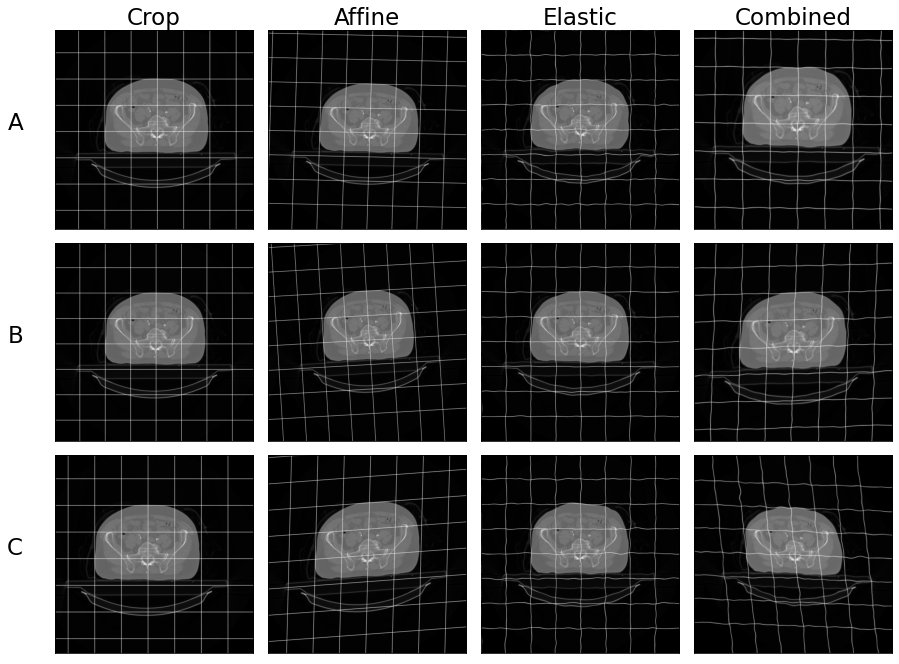
\includegraphics[width=1\textwidth]{figures/augment}
		\caption{Training data augmentation for single input image with random sampling of parameters: image crop and resize, affine transformation, elastic deformation, and combined transformations. Each matching contour set is augmented under an identical transformation. An individual transformation type has $P_{val}=0.33$ of occurring. Additional augmentations not shown: Left/right inversion and Gaussian noise}
		\label{fig:augment}
	\end{center}
\end{figure}

\section{Model architecture}
\label{ch:method-architecture}
We designed a 2D U-net architecture with 7 levels, consisting of 6 encoding and 6 decoding blocks, outlined in Figure \ref{fig:model}. The model accepts a full resolution (512 x 512) CT image as input, and outputs selected contours in the original resolution by the use of padded convolutions, each of which is followed by batch normalisation and ReLU activation. Each encoding block performs a repeated sequence of 3 x 3 convolution (increasing feature channels). Extracted feature maps are passed via the skip connection in one pathway, while a 3 x 3 convolution with stride size 2 halves the resolution before passing features to the next encoding block.

Conversely, each decoding block upsamples input via a 3 x 3 2D transposed convolution with stride size of 2. Upsampled feature maps are then concatenated with skip connections. Dropout is selectively performed with a probability value of 20\%, before additional 3 x 3 convolution sequences reduce the feature channels.

Finally, multi-organ segmentation can be controlled via the C (Channel - corresponding to the number of segmentations) output variable specified in the last 1 x 1 convolutional layer. A sigmoid activation function is used to account for the non-mutually exclusive nature of pixel-wise binary classification on anatomic structures (i.e. a voxel can belong to multiple structures).

\begin{figure}[!htb]
	\begin{center}
		\hspace*{-1.3cm}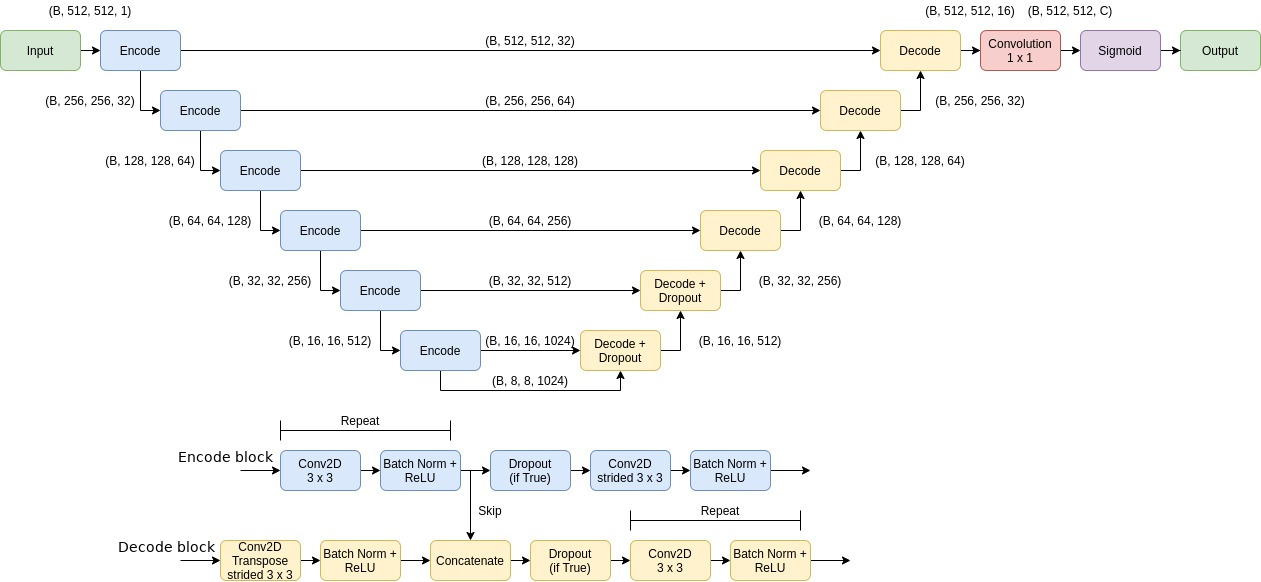
\includegraphics[width=1.15\textwidth]{figures/model_diagram}
		\caption{Modified 2D U-net architecture: Composed of encoding (blue) and decoding blocks (yellow). MaxPooling layers replaced by strided convolution. Added batch normalisation and final sigmoid activation.Tensor dimensions (Batch size, X, Y, Channels) are included for each connection. Internal layers of encoding blocks (blue) and decoding blocks (yellow) are included under the high-level overview.}
		\label{fig:model}
	\end{center}
\end{figure}

The model was trained using the Adam (Adaptive momentum estimation) optimisation algorithm \cite{kingma2014} with an initial learning rate of $10^{-5}$, a batch size of 1 for pelvic imaging, and 3 for canine imaging. Model training was scheduled to conclude when validation loss had not improved for a period of 20 epochs. In addition, learning rate decay was triggered by a validation loss plateau period of 3 epochs. Initial model weights were determined via `He' kernel initialisation), which samples from a zero mean Gaussian distribution with variance $\sigma=\sqrt{2/N}$ (as in Ronneberger et al \cite{Ronneberger_2015}), where N is the incoming nodes for a single activation (i.e. for n x n convolution over M feature maps, N = n x n x M). In addition, we accelerate training for pelvic imaging by adopting the strategy of Bertels et. al to further initialising model parameters via 3 epochs of training with binary cross entropy.



\section{Loss functions}
\label{ch:method-loss}
A total of 5 loss functions were assessed for pelvic imaging: Binary Cross entropy (BCE), soft dice similarity coefficient (soft DSC) \cite{Bertels2019}, weighted soft dice similarity coefficient (w. soft DSC or modified generalised dice loss \cite{Sudre_2017}), a modified combination loss BCE + 2 (w. soft DSC) \cite{taghanaki2018}, and focal Tversky loss \cite{Zhu_2018, Khan2019, abraham2018}. In contrast, weighted soft DSC was not attempted for canine imaging due to the single segmentation output.

Calculations for weighted soft DSC were performed via equation \ref{eq:method_wsdsc}, with component equations presented in \ref{eq:w}, \ref{eq:i}, and \ref{eq:u}. $W$, $I$, and $U$ correspond to the weight, intersection and union vectors, indexed with respect to each contour structure by $k\in\{1,...,n\}$; while $\epsilon$ represents a small value $>0$ to ensure division is defined. In addition, $|\cdot|$ notation refers to the cardinality of a set (i.e. the total number of pixels in a contour mask - including zeros), while $t_{k}$ refers to a ground truth array, $p_{k}$ to the predicted array, and $\odot$ to the Hadamard product. The standard soft DSC can be implemented by setting weights $W=\vec{1}$.  Code required for a tensorflow implementation is included in the pymedphys library.

\begin{equation}
w. \, soft \, DSC = \frac{2 \, (W \cdot I + \epsilon)}{W \cdot U + \epsilon}
\label{eq:method_wsdsc}
\end{equation}

\begin{equation}
W = (W_{1}, ..., W_{n}) \; \; \textbf{:} \; \; W_{k} = \frac{\sum_{k=1}^{n} |t_{k} |}{t_{k} + \epsilon}
\label{eq:w}
\end{equation}

\begin{equation}
%I = (I_{1}, ..., I_{n}) \; \; \textbf{:} \; \; I_{i} = \langle\,t_{i} \,,\,  p_{i}\,\rangle
I = (I_{1}, ..., I_{n}) \; \; \textbf{:} \; \; I_{k} = \sum_{i,j=1}(t_{k} \, \odot \,  p_{k})_{ij}
\label{eq:i}
\end{equation}

\begin{equation}
U = (U_{1}, ..., U_{n}) \; \; \textbf{:} \; \; U_{k} =  \sum_{i,j=1}(t_{k} + p_{k})_{ij}
\label{eq:u}
\end{equation}

\todo[inline, color=blue!40]{Addition? - Tversky loss formula and parameters used - \cite{abraham2018}}

Final model performance was evaluated on an independent test dataset via both DSC and sDSC metrics. Organ specific tolerance $\tau$ for rectum and bladder contours were taken as the 95th percentile absolute mean surface distance in mm between expert observers from Roach et al. \cite{Roach_2019}. MSD$_{95}$ values calculated from Roach et al. show organ-specific tolerances of 1.46 mm for the bladder, and 6.99 mm for the rectum.